% This file was created by tikzplotlib v0.9.2.
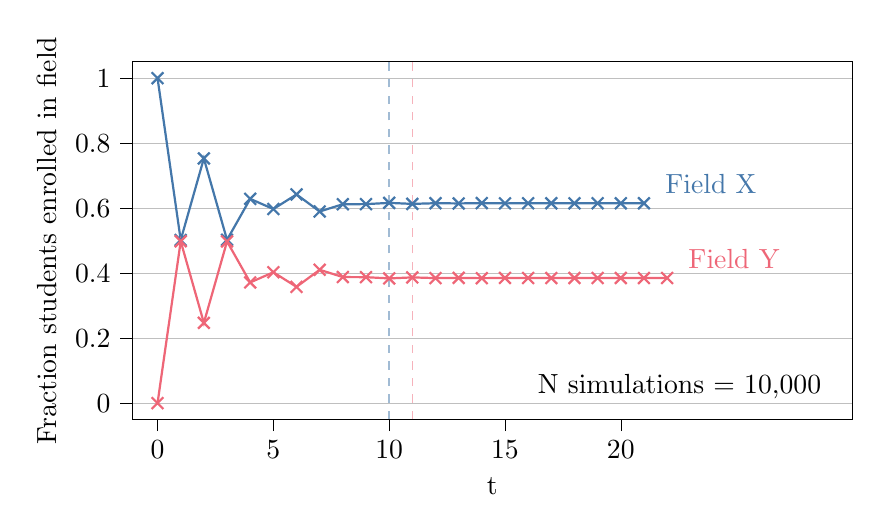
\begin{tikzpicture}

\definecolor{color0}{rgb}{0.266666666666667,0.466666666666667,0.666666666666667}
\definecolor{color1}{rgb}{0.933333333333333,0.4,0.466666666666667}

\begin{axis}[
height=6.121302808757603cm,
tick align=outside,
tick pos=left,
unbounded coords=jump,
width=10.729849cm,
x grid style={white!69.0196078431373!black},
xlabel={t},
xmin=-1.1, xmax=30,
xtick style={color=black},
xtick={0,5,10,15,20},
xticklabels={\(\displaystyle 0\),\(\displaystyle 5\),\(\displaystyle 10\),\(\displaystyle 15\),\(\displaystyle 20\)},
ylabel={Fraction students enrolled in field},
ymajorgrids,
ymin=-0.05, ymax=1.05,
ytick style={color=black},
ytick={0,0.2,0.4,0.6,0.8,1},
yticklabels={\(\displaystyle 0\),\(\displaystyle 0.2\),\(\displaystyle 0.4\),\(\displaystyle 0.6\),\(\displaystyle 0.8\),\(\displaystyle 1\)}
]
\addplot [thick, color0, mark=x, mark size=3, mark options={solid}]
table {%
0 1
1 0.5019
2 0.753
3 0.5025
4 0.6286
5 0.5973
6 0.6422
7 0.5897
8 0.6121
9 0.6124
10 0.6162
11 0.6131
12 0.6152
13 0.6145
14 0.6155
15 0.6147
16 0.615
17 0.6151
18 0.6149
19 0.6151
20 0.615
21 0.6151
22 nan
};
\addplot [thick, color1, mark=x, mark size=3, mark options={solid}]
table {%
0 0
1 0.4981
2 0.247
3 0.4975
4 0.3714
5 0.4027
6 0.3578
7 0.4103
8 0.3879
9 0.3876
10 0.3838
11 0.3869
12 0.3848
13 0.3855
14 0.3845
15 0.3853
16 0.385
17 0.3849
18 0.3851
19 0.3849
20 0.385
21 0.3849
22 0.3849
};
\addplot [semithick, color0, opacity=0.5, dashed]
table {%
10 -0.05
10 1.05
};
\addplot [semithick, color1, opacity=0.5, dashed]
table {%
11 -0.05
11 1.05
};
\draw (axis cs:21.5,0.6451) node[
  anchor=base west,
  text=color0,
  rotate=0.0
]{Field X};
\draw (axis cs:22.5,0.4149) node[
  anchor=base west,
  text=color1,
  rotate=0.0
]{Field Y};
\draw (axis cs:16,0.03) node[
  anchor=base west,
  text=black,
  rotate=0.0
]{N simulations = 10,000};
\end{axis}

\end{tikzpicture}
